\documentclass[11pt, dvipsnames, handout]{beamer}
\newtoggle{full}
\settoggle{full}{true}

\newtoggle{covered}
\settoggle{covered}{false}

\newtoggle{presentable}
\settoggle{presentable}{false}

\newtoggle{dualscreen}
\settoggle{dualscreen}{false}

\usepackage{pgfplots}
%\pgfplotsset{compat = newest}

\usepackage{pgfpages}

\setbeamertemplate{note page}{\pagecolor{yellow!5}\vfill \insertnote \vfill}
\usepackage{collect}
\definecollection{notes}
\newcounter{notestaken}

\usepackage{xpatch}

\usepackage{ulem}

\usepackage[framemethod=tikz]{mdframed}

\usepackage{scalerel}
\usepackage{calc}

%\usepackage{enumitem}
\setlength\fboxsep{.2em}

\usepackage{graphicx} % Allows including images
\usepackage{booktabs} % Allows the use of \toprule, \midrule and \bottomrule in tables

\xpatchcmd{\itemize}
  {\def\makelabel}
  {\setlength{\itemsep}{0.65 em}\def\makelabel}
  {}
  {}


\xpatchcmd{\beamer@enum@}
  {\def\makelabel}
  {\setlength{\itemsep}{0.65 em}\def\makelabel}
  {}
  {}


%\makeatletter
%\renewcommand{\itemize}[1][]{%
%  \beamer@ifempty{#1}{}{\def\beamer@defaultospec{#1}}%
%  \ifnum \@itemdepth >2\relax\@toodeep\else
%    \advance\@itemdepth\@ne
%    \beamer@computepref\@itemdepth% sets \beameritemnestingprefix
%    \usebeamerfont{itemize/enumerate \beameritemnestingprefix body}%
%    \usebeamercolor[fg]{itemize/enumerate \beameritemnestingprefix body}%
%    \usebeamertemplate{itemize/enumerate \beameritemnestingprefix body begin}%
%    \list
%      {\usebeamertemplate{itemize \beameritemnestingprefix item}}
%      {%
%        \setlength\topsep{1em}%NEW
%        \setlength\partopsep{1em}%NEW
%        \setlength\itemsep{1em}%NEW
%        \def\makelabel##1{%
%          {%
%            \hss\llap{{%
%                \usebeamerfont*{itemize \beameritemnestingprefix item}%
%                \usebeamercolor[fg]{itemize \beameritemnestingprefix item}##1}}%
%          }%
%        }%
%      }
%  \fi%
%  \beamer@cramped%
%  \raggedright%
%  \beamer@firstlineitemizeunskip%
%}
%
%
%
%
%
%\makeatother

%\setlist[beamer@enum@]{topsep=1 em}
%\let\origcheckmark\checkmark %screw you dingbat
%\let\checkmark\undefined %screw you dingbat
%\usepackage{dingbat} 
%\let\checkmark\origcheckmark %screw you dingbat






%\usepackage{fontawesome}

\usepackage{mathtools}
\usepackage{etoolbox, calculator}

\usepackage{xcolor}
\usepackage{tikz}
\usetikzlibrary{arrows.meta}
\usetikzlibrary{calc}
\usepackage[nomessages]{fp}
\usepackage{transparent}
\usepackage{accsupp}
%\usepackage{color, xcolor}

%colorblind-friendly palette
%\definecolor{dblue}{RGB}{51,34,136}
\definecolor{lblue}{RGB}{136,204,238}
%\definecolor{green}{RGB}{17,119,51}
\definecolor{tan}{RGB}{221,204,119}
%\definecolor{mauve}{RGB}{204,102,119}

\usepackage{tcolorbox}



\usepackage{xifthen}
\usepackage{nicefrac}
\usepackage{amsmath}
\usepackage{amsthm}
\usepackage{amssymb}
\theoremstyle{definition}
\newtheorem*{define}{Definition}
\newtheorem*{recall}{Recall}


\DeclareMathOperator{\tr}{tr}

\usepackage{multicol}
%\setlength{\columnsep}{1cm}

\usepackage{tablists, amsmath,vwcol, cancel, polynom}
\usetikzlibrary{shapes, patterns, decorations.shapes}
%\usepackage{tikzpeople}
\tikzstyle{vertex}=[shape=circle, minimum size=2mm, inner sep=0, fill]
\tikzstyle{opendot}=[shape=circle, minimum size=2mm, inner sep=0, fill=white, draw]

% common math quick commands
\newcommand{\nicedd}[2]{\nicefrac{\text{d}#1}{\text{d}#2}}
\newcommand{\dd}[2]{\dfrac{\text{d}#1}{\text{d}#2}}
\newcommand{\pd}[2]{\dfrac{\partial #1}{\partial#2}}
\renewcommand{\d}[1]{\text{d}#1}
\newcommand{\ddn}[3]{\dfrac{\text{d}^{#3}#1}{\text{d}#2^{#3}}}
\newcommand{\pdn}[3]{\dfrac{\partial^{#3}#1}{\partial#2^{#3}}}
\newcommand{\p}[0]{^{\prime}}
\newcommand{\pp}[0]{^{\prime\prime}}
\newcommand{\op}[2][\text{L}]{#1 \left[ #2 \right]}

\newcommand{\lap}[1]{\mathcal{L}\left\{#1\right\}}
\newcommand{\lapinv}[1]{\mathcal{L}^{-1}\left\{#1\right\}}
\newcommand{\lapint}[1]{\int_0^\infty e^{-st}#1dt}
\newcommand{\evalat}[2]{\Big|_{#1}^{#2}}

\newcommand{\paren}[1]{ \left( #1 \right)}

\newcommand{\haxis}[4][\normcolor]{\draw[#1, <->] (-#2,0)--(#3,0) node[right]{$#4$}; }


\newcommand{\axis}[4]{\draw[\normcolor, <->] (-#1,0)--(#2,0) 
node[right]{$x$};
\draw[help lines, <->] (0,-#3)--(0,#4) node[above]{$y$};}

\newcommand{\laxis}[6]{\draw[<->] (-#1,0)--(#2,0) 
node[right]{$#5$};
\draw[ <->] (0,-#3)--(0,#4) node[above]{$#6$};}
\newcommand{\xcoord}[2]{
	\draw (#1,.2)--(#1,-.2) node[below]{$#2$};}
\newcommand{\textnode}[3]{
	\draw (#1,#2) node[below]{$#3$};}
	
\newcommand{\nxcoord}[2]{
	\draw (#1,-.2)--(#1,.2) node[above]{$#2$};}
\newcommand{\ycoord}[2]{
	\draw (.2,#1)--(-.2,#1) node[left]{$#2$};}
\newcommand{\nycoord}[2]{
	\draw (-.2,#1)--(.2,#1) node[right]{$#2$};}
\newcommand{\dlim}{\displaystyle\lim}
\newcommand{\dlimx}[1]{\displaystyle\lim_{x \rightarrow #1}}
\newcommand{\stickfig}[2]{
	\draw (#1,#2) arc(-90:270:2mm);
	\draw (#1,#2)--(#1,#2-.5) (#1-.25,#2-.75)--(#1,#2-.5)--(#1+.25,#2-.75) (#1-.2,#2-.2)--(#1+.2,#2-.2);}	

%\newcounter{example}
%\setcounter{example}{1}
%\newcounter{preFrameExample}
%\AtBeginEnvironment{frame}{\setcounter{preFrameExample}{\value{example}}}
%\newcommand{\ex}[1]{
%	 \setcounter{example}{\value{preFrameExample}}
%	 \textcolor{green}{\small\fbox{Example \arabic{example}: #1}}\\[8pt]
%	\stepcounter{example}}
%\newcommand{\exans}[1]{
%	\SUBTRACT{\value{preFrameExample}}{1}{\n}
%	 \textcolor{green}{\small\fbox{Solution \n: #1}}\\[8pt]}
\mode<presentation> {

% The Beamer class comes with a number of default slide themes
% which change the colors and layouts of slides. Below this is a list
% of all the themes, uncomment each in turn to see what they look like.


\usetheme{CambridgeUS}
\usecolortheme[named=black]{structure}


\newcommand{\studentcolor}[0]{ForestGreen}
\newcommand{\normcolor}[0]{NavyBlue}
\newcommand{\alertcolor}{Red}

\setbeamercolor{normal text}{fg=\normcolor}
\setbeamercolor{frametitle}{fg=\normcolor}
\setbeamercolor{section in head/foot}{fg=Black, bg=Gray!20}
\setbeamercolor{subsection in head/foot}{fg=Green!70!Black, bg=Gray!10}
\setbeamercolor{alerted text}{fg=\alertcolor}
\setbeamerfont{alerted text}{series=\bf}
\setbeamertemplate{enumerate items}[default]
\setbeamercolor{enumerate item}{fg=\normcolor}

\setbeamertemplate{footline} % To remove the footer line in all slides uncomment this line
%\setbeamertemplate{footline}[page number] % To replace the footer line in all slides with a simple slide count uncomment this line

\setbeamertemplate{navigation symbols}{} % To remove the navigation symbols from the bottom of all slides uncomment this line
}

\newcommand{\alertbox}[1]{\tcbox[on line, colframe=\alertcolor, colback=White, left=2pt,right=2pt,top=2pt,bottom=2pt]{\usebeamercolor*{normal text}#1}}


\newcommand{\startstu}{\setbeamercolor{normal text}{fg=\studentcolor}\usebeamercolor*{normal text}\setbeamercolor{enumerate item}{fg=\studentcolor}\usebeamercolor*{enumerate item}}
\newcommand{\stopstu}{\setbeamercolor{normal text}{fg=\normcolor}\usebeamercolor*{normal text}\setbeamercolor{enumerate item}{fg=\normcolor}\usebeamercolor*{enumerate item}}

\newcommand{\takenote}[1]{ \begin{collect}{notes}{}{}{}{}  #1  \end{collect}  \addtocounter{notestaken}{1}} %\ifthenelse{\value{notestaken}>0}{\hrulefill\\}{}

\makeatletter
\newcommand{\cover}{\alt{\beamer@makecovered}{\beamer@fakeinvisible}}
\newcommand{\ucover}[1]{\iftoggle{full}{}{\beamer@endcovered}\stopstu#1\startstu\iftoggle{full}{}{\beamer@startcovered}}
\makeatother

\newcommand{\skippause}{ \addtocounter{beamerpauses}{-1}}
\newcommand{\blockpres}{ \skippause \pause }

\newcommand{\studentify}[1]{\startstu #1  \stopstu }
\newcommand{\student}[1]{\iftoggle{full}{ \pause  \studentify{#1} }{\iftoggle{covered}{\studentify{#1}}{\cover{  #1 }}}}
\newcommand{\cstudent}[1]{\student{\begin{center} #1 \end{center}}}
\newcommand{\fullonly}[1]{\iftoggle{full}{ #1}{}}
\newcommand{\presentonly}[1]{\iftoggle{presentable}{ #1}{}}

\usepackage{xparse}
\usepackage{xifthen}

% shortcuts for commonly-used presentation elements
%\NewDocumentCommand{\slide}{o m}
% {\IfValueTF{#1}{\begin{frame}[t]{#1}}{\begin{frame}[t]} #2 \end{frame}}

\newtoggle{iscovered}

\newcommand{\slide}[2][]{%
%\setcounter{notestaken}{0}
\takenote{#2} 
%\ifthenelse{\equal{#1}{}}{\begin{frame}[t]}{\begin{frame}[t]{#1}} #2 \ifthenelse{\value{notestaken}>0}{ \note{\includecollection{notes}}}{} \end{frame}%
\ifthenelse{\equal{#1}{}}{\begin{frame}[t]}{\begin{frame}[t]{#1}} #2 \iftoggle{covered}{\settoggle{iscovered}{true}}{\settoggle{iscovered}{false}}  \note{ \iftoggle{iscovered}{}{\settoggle{covered}{true}} #2 \iftoggle{iscovered}{}{\settoggle{covered}{false}} } \end{frame}%
%\setcounter{notestaken}{0}
}
\newcommand{\defn}[2][]{%
 \setcounter{listcounter}{0}%
\ifthenelse{\equal{#1}{}}{\begin{block}{Definition}}{\begin{block}{#1 :}}%
 #2 \vspace{0.25em} \ifthenelse{\value{listcounter}>0}{\skippause}{} \pause \end{block}%
}



\newcommand{\arr}[2]{\begin{array}{#1}#2\end{array}}
\newcommand{\mat}[2]{\left[\arr{#1}{#2}\right]}
\newcommand{\carray}[1]{\arr{c}{#1}}
\newcommand{\larray}[1]{\arr{l}{#1}}
\newcommand{\rarray}[1]{\arr{r}{#1}}
\newcommand{\colvec}[1]{\mat{c}{#1}}

\newcommand{\itmz}[1]{\addtocounter{listcounter}{1} \begin{itemize}#1 \end{itemize} }
\newcommand{\subitem}[1]{\addtocounter{listcounter}{1} \begin{itemize} \item #1 \end{itemize}}
%
\newcommand{\enum}[1]{\addtocounter{listcounter}{1} \begin{enumerate} #1  \end{enumerate}  }


\newcommand{\algnlbl}[1]{\begin{align}#1  \end{align}} 
\newcommand{\algn}[1]{\begin{align*}#1  \end{align*}} 
\newcommand{\lgn}[1]{ \action<+->{#1} }
\newcommand{\slgn}[1]{\iftoggle{full}{\action<+->{ \startstu #1 \stopstu}}{ \cover{ #1 } } \takenote{$#1$}}

\newcommand{\chckmrk}{\alert{\checkmark}}

\usepackage{pifont}
\newcommand{\xmark}{\alert{\text{\large \ding{55}}}}

\newcommand{\return}[0]{\raisebox{.5ex}{\rotatebox[origin=c]{180}{$\Lsh$}}}
\usepackage{pbox}
%\newcommand{\ex}[1]{\rotatebox[origin=c]{10}{\uline{ex}}:$\;$\pbox[t][][b]{0.9\linewidth}{#1}}
\newcommand{\ex}[1]{\uline{ex}:$\;$\pbox[t][][t]{0.9\linewidth}{#1}}
\newcommand{\eg}[1]{e.g.,$\;$\pbox[t][][t]{0.9\linewidth}{#1}}
\newcommand{\tikzplot}[8][]{%
\begin{tikzpicture}

\begin{scope}[]%
\clip(-#2,-#4) rectangle (#3,#5);%
#8%
\end{scope}%
\laxis{#2}{#3}{#4}{#5}{#6}{#7}%
#1
\end{tikzpicture}%
}


\newcommand{\cancelslide}[1]{%
\begingroup%
\setbeamertemplate{background canvas}{%
\begin{tikzpicture}[remember picture,overlay]%
\draw[line width=2pt,red!60!black] %
  (current page.north west) -- (current page.south east);%
\draw[line width=2pt,red!60!black] %
  (current page.south west) -- (current page.north east);%
\end{tikzpicture}}%
#1%
\endgroup%
}
\renewcommand{\CancelColor}{\color{red}}
\newcommand{\twocols}[3][0.5]{\begin{columns}\begin{column}{#1\textwidth}#2\end{column}\hspace{1em}\vrule{}\hspace{1em}\begin{column}{#1\textwidth}#3\end{column}\end{columns}}

\newcommand{\twomini}[5][1]{\calculatespace \begin{minipage}[t]{\columnwidth}\begin{minipage}[][#1\contentheight][t]{#2\columnwidth}#4\end{minipage}\hfill\begin{minipage}[][#1\contentheight][t]{#3\columnwidth}#5\end{minipage}\end{minipage}}

\newcommand{\threemini}[7][1]{\calculatespace \begin{minipage}[t]{\columnwidth}\begin{minipage}[][#1\contentheight][t]{#2\columnwidth}#5\end{minipage}\hfill\begin{minipage}[][#1\contentheight][t]{#4\columnwidth}#6\end{minipage}\hfill\begin{minipage}[][#1\contentheight][t]{#3\columnwidth}#7\end{minipage}\end{minipage}}


\newcounter{listcounter}
\setcounter{listcounter}{0}



\newif\ifsidebartheme
\sidebarthemetrue

\newdimen\contentheight
\newdimen\contentwidth
\newdimen\contentleft
\newdimen\contentbottom
\makeatletter
\newcommand*{\calculatespace}{%
\contentheight=\paperheight%
\ifx\beamer@frametitle\@empty%
    \setbox\@tempboxa=\box\voidb@x%
  \else%
    \setbox\@tempboxa=\vbox{%
      \vbox{}%
      {\parskip0pt\usebeamertemplate***{frametitle}}%
    }%
    \ifsidebartheme%
      \advance\contentheight by-1em%
    \fi%
  \fi%
\advance\contentheight by-\ht\@tempboxa%
\advance\contentheight by-\dp\@tempboxa%
\advance\contentheight by-\beamer@frametopskip%
\ifbeamer@plainframe%
\contentbottom=0pt%
\else%
\advance\contentheight by-\headheight%
\advance\contentheight by\headdp%
\advance\contentheight by-\footheight%
\advance\contentheight by4pt%
\contentbottom=\footheight%
\advance\contentbottom by-4pt%
\fi%
\contentwidth=\paperwidth%
\ifbeamer@plainframe%
\contentleft=0pt%
\else%
\advance\contentwidth by-\beamer@rightsidebar%
\advance\contentwidth by-\beamer@leftsidebar\relax%
\contentleft=\beamer@leftsidebar%
\fi%
}
\makeatother



\iftoggle{dualscreen}{\setbeameroption{show notes on second screen=right}}{}


\begin{document}
\section{Lecture 17}
\subsection{Laplace Transforms Practice}

\slide[Laplace Inversion Tactics]{\small
\enum{
\item Function has denominator that can factor.
\subitem{factor and use partial fraction decomposition}
\[\frac{1}{(s+a)s}=\frac{1}{as}-\frac{1}{a(s+a)} \quad \underrightarrow{\mathcal{L}^{-1}}\quad  \frac{1}{a}-\frac{1}{a}e^{-at}\]
\item Denominator has something with $(s-a)^n$ but numerator has $s$ appearing in it, not $s-a$. \vfill
\subitem{Split numerator by adding/subtracting so that all appearances of $s$ are in the form $s-a$ \item use First Shift Theorem to invert}\[\frac{s}{(s-a)^n}=\frac{s-a}{(s-a)^n}+\frac{a}{(s-a)^n} \quad \underrightarrow{\mathcal{L}^{-1}}\quad \frac{e^{at}t^{n-2}}{(n-2)!}+\frac{a}{(n-1)!}e^{at}t^{n-1}\]\vfill
\item Numerator has incorrect constant $A$ for inversion. \subitem{Mulitply by $\frac{\omega}{\omega}$ and swap $\omega$ with $A$ :\[\frac{\omega}{\omega}\frac{A}{\omega^2+s^2}=\frac{A}{\omega}\frac{\omega}{\omega^2+s^2}\quad \underrightarrow{\mathcal{L}^{-1}}\quad   \frac{A}{\omega}\sin(\omega t) \] }
}
}

\slide{\ex{$y\pp+2y\p+5y=0$, \quad $y(0)=y_0$, $y\p(0)=v_0$}
\student{
\algn{s^2Y(s)-&sy_0-v_0+2sY(s)-2y_0+5Y(s)=0\\
Y(s)&=\frac{sy_0+v_0+2y_0}{s^2+2s+5}=\frac{sy_0+v_0+2y_0}{\underbrace{s^2+2s+1}_{(s+1)^2}\underbrace{-1+5}_{2^2}}\\
&=\frac{sy_0+v_0+2y_0}{(s+1)^2+2^2 } =\frac{sy_0}{(s+1)^2+2^2 } + \frac{v_0+2y_0}{(s+1)^2+2^2 }\\
&=y_0 \lap{e^{-t}\underbrace{\lapinv{\frac{s}{s+2^2}}}_{\cos(2t)}}+(v_0+y_0 )\lap{e^{-t} \underbrace{\lapinv{\frac{1}{s^2+2^2}}}_{\frac12 \sin(2t)}}\\\\
y(t)&=y_0e^{-t}\cos(2t)+\frac{v_0+y_0}{2}e^{-t}\sin(2t)} 
}
}%end slide

\slide{\ex{$y\pp+12y\p+36y=0$, \quad $y(0)=y_0$, $y\p(0)=v_0$}

\student{
\algn{s^2Y(s)-&sy_0-v_0+12sY(s)-12y_0+36Y(s)=0\\
Y(s)&=\frac{sy_0+v_0+12y_0}{s^2+12s+36}=\frac{sy_0+v_0+12y_0}{(s+6)^2}\\
&=\frac{y_0\cancel{(s+6)}}{(s+6)^{\cancel{2}}}+\frac{v_0+12y_0-6y_0}{(s+6)^2}\\
&=y_0\underbrace{\frac{1}{s+6}}_{\lap{e^{-6t}}}+(v_0+6y_0) \frac{1}{(s+6)^2}\\
&=y_0\lap{e^{-6t}}  +(v_0+6y_0) \lap{e^{-6t} \lapinv{\frac{1}{s^2}}}\\\\
y(t)&=y_0e^{-6t}+(v_0+6y_0)e^{-6t}t} 
}

}%end slide

\slide{\ex{$y\p+6y=u_1(t)\student{=\begin{cases}
0 & t<1\\
1 & t\geq1
\end{cases}}$}
\student{\twomini[.55]{.6}{.3}{\algn{ sY-&y_0+6Y=\frac{e^{-s}}{s}\\
Y&=\frac{\frac{e^{-s}}{s}+y_0}{s+6}=\frac{e^{-s}}{s(s+6)}+\frac{y_0}{s+6}\\
Y(s)&=\frac{1}{6}\frac{e^{-s}}{s}-\frac{1}{6}\frac{e^{-s}}{s+6}+\frac{y_0}{s+6}\\
& \downarrow \mathcal{L}^{-1}\\
y(t)&=\frac16 u(t-1)-\frac16 e^{-6(t-1)} u(t-1)+y_0e^{-6t}
}\vfill}{$\frac{1}{s(s+6)}=\frac{A}{s}+\frac{B}{s+6}$\\~\\$\Rightarrow 1=A(s+6)+Bs $\\~\\$\Rightarrow \arr{l}{1=6A\\0=A+B}$ \\~\\$\Rightarrow \arr{l}{A=\frac16\\B=-\frac16}$ \vfill}}
\tikzplot[
\student{\xcoord{3}{1} \ycoord{1.25}{\frac16}}
]{.1}{10}{.1}{1.5}{t}{y(t)}{
\student{
\draw[domain=0:2, thick, samples=100] plot ({\x*1.5}, {.8*exp(-\x)});
\draw[domain=2:10, thick, samples=100] plot ({\x*1.5}, {.8*exp(-\x)+(1-exp(-(\x-2)))*1.25});
\draw[domain=0:10, thick, dashed, samples=100] plot ({\x*1.5}, {1.25});
}}
}

\slide{\ex{$y\pp+2y\p+5y=u_5(t)-u_{15}(t)$, \quad $y(0)=y_0$, $y\p(0)=v_0$}
\student{
\algn{s^2Y(s)-&sy_0-v_0+2sY(s)-2y_0+5Y(s)=\frac{e^{-5s}}{s} - \frac{e^{-15s}}{s}\\
Y(s)&= \frac{  \paren{\frac{e^{-s}}{s} - \frac{e^{-2s}}{s}} + sy_0+v_0+2y_0}{s^2+2s+5}\\
&=  \paren{ e^{-5s} - e^{-15s}}  \underbrace{\frac{ 1}{s(s^2+2s+5)}}_{F(s)}+   \underbrace{\frac{ 1}{s^2+2s+5}}_{\text{homogeneous part}}\\\\
y(t)&=u_5(t)\left[ \lapinv{F(s)} \right]_{t=t-5}\\
&\phantom{=} - u_{15}(t)\left[ \lapinv{F(s)} \right]_{t=t-15}\\
&\phantom{=} + y_0e^{-t}\cos(2t)+\frac{v_0+y_0}{2}e^{-t}\sin(2t)
}
}
}%end slide

\slide{$\lapinv{\frac{1}{s(s^2+2s+5)}}=\;???$ 

\student{
\algn{F(s)=\frac{1}{s(s^2+2s+5)} & = \frac{A}{s} +\frac{Bs+C}{s^2+2s+5}\\
1&=As^2+2As+5A + Bs^2+Cs\\
\text{constant terms: } 1&= 5A \qquad \Rightarrow A=\frac15 \\
\text{$s$ terms: } 0 &= 2A+C   \qquad \Rightarrow C=-2A=-\frac25\\
\text{$s^2$ terms: } 0 &=	A+B  \qquad \Rightarrow B=-A=-\frac15\\
F(s) &= \frac{1}{5s} - \frac15 \frac{s+2}{(s+1)^2+2^2}\\
&=  \frac{1}{5s} -  \frac15 \paren{\frac{s+1}{(s+1)^2+2^2}  - \frac{1}{(s+1)^2+2^2}}  \\
f(t) &= \frac15 \paren{1-e^{-t}\paren{cos(2t) -\frac12 \sin(2t)}}}
}
}

\slide{
\algn{y(t)&=u_5(t)\frac15 \paren{1-e^{-(t-5)}\paren{cos(2(t-5)) -\frac12 \sin(2(t-5))}}\\
&\phantom{=} - u_{15}(t)u_5(t)\frac15 \paren{1-e^{-(t-15)}\paren{cos(2(t-15)) -\frac12 \sin(2(t-15))}}\\\
&\phantom{=} + y_0e^{-t}\cos(2t)+\frac{v_0+y_0}{2}e^{-t}\sin(2t)}

\centerline{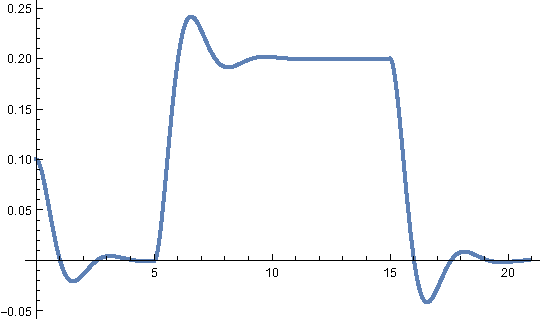
\includegraphics[width=9cm]{images/Heaviside_jiggle.pdf}}
}

\slide{\ex{$y\pp+y\p=1$, $y(0)=y_0$, $y\p(0)=v_0$}
\student{\vspace{-.5em}
\algn{s^2Y(s)-&sy_0-v_0+sY(s)-y_0=\frac1s\\
(s^2+s)Y&=sy_0+y_0+v_0+\frac1s\\
Y(s)&=\frac{\cancel{s}y_0}{\cancel{s}(s+1)}+\frac{y_0+v_0}{s(s+1)}+\frac{1}{s^2(s+1)}}\vspace{-1.5em}
\algn{\frac{1}{s(s+1)}&=\frac{A}{s}+\frac{B}{s+1}&\arr{r}{1=A(s+1)+Bs\\A=1, B=-1}\\
&=\frac1s-\frac{1}{s+1}\\
\frac{1}{s^2(s+1)}&=\frac{A}{s^2}+\frac{B}{s}+\frac{C}{s+1}&\arr{r}{1=A(s+1)+Bs(s+1)+Cs^2\\\uline{s=0:}\;A=1,\quad  \uline{s=-1:}\;C=1}\\
&=\frac{1}{s^2}-\frac{1}{s}+\frac{1}{s+1}&\uline{s=1:}\; 2+2B+\cancel{1}=\cancel{1}}\vspace{-1.5em}
\algn{Y(s)&=\cancel{\frac{y_0}{s+1}}+\frac{y_0+v_0}{s}-\frac{\cancel{y_0}+v_0}{s+1}+\frac{1}{s^2}-\frac{1}{s}+\frac{1}{s+1}&B=-1}
}
}%end slide

\slide{continuing $\dots Y(s)=\frac{y_0+v_0-1}{s}+\frac{1-v_0}{s+1}+\frac{1}{s^2}$
\student{\algn{y(t)&=y_0+v_0+1+(1-v_0)e^{-t}+t\\
&=\underbrace{c_1+c_2e^{-t}}_{y_h}+\underbrace{t}_{y_p}\intertext{\uline{M.U.C.}}
y\pp+y\p&=1\intertext{homogeneous problem}
&r^2+r=0\Rightarrow r(r+1)=0 &\Rightarrow y_h=c_1+c_2e^{-t} \intertext{RHS in nullspace of operator}
y_p=Bt \dots}
put it all together and then solve for $c_1$ and $c_2\dots$
}

}%end slide


\end{document}
